\section{Which meeting risks does the expiry calendar identify?}\label{sec:calendar}
\subsection{The observed panel}
Suppose the observed expiries are $0<S_1<\cdots<S_L$. Expiry $S_\ell$ may refer to its own accrual window $[a_\ell,b_\ell]$, but assume $S_\ell<a_\ell$ throughout. Divide its fitted log variance by $\delta_\ell^2$, where $\delta_\ell=b_\ell-a_\ell$, to obtain $\cV(S_\ell)$. In this section these quantities are observed exactly.

Represent the background variance rate by $n_b$ nonnegative parameters. Fix $0=c_0<c_1<\cdots<c_{n_b}$, with $c_{n_b}\geq S_L$, and set $\sigma(s)^2=u_j$ on $[c_{j-1},c_j)$, with $\sigma=0$ after $c_{n_b}$. The parameter vector is
\[
\theta=(v_1,\ldots,v_N,u_1,\ldots,u_{n_b})^\top\geq0.
\]
For an interval $J$, let $\mathfrak l_j(J)$ be the length of its intersection with $[c_{j-1},c_j)$. The observed vector $\boldsymbol{\cV}=(\cV(S_1),\ldots,\cV(S_L))^\top$ satisfies
\begin{equation}\label{eq:panel}
\boldsymbol{\cV}=\mathsf A\theta,\qquad
\mathsf A_{\ell i}=\ind_{\{T_i\leq S_\ell\}},\qquad
\mathsf A_{\ell,N+j}=\mathfrak l_j((0,S_\ell]).
\end{equation}
Thus calibration of these observations is a nonnegative linear inverse problem. The restriction $\sigma=0$ after $c_{n_b}$ completes the model outside the panel horizon; observations through $S_L$ provide no evidence for that tail restriction. The columns for meetings record whether each meeting has occurred by an expiry. The remaining columns record the exposure to each background-variance interval.

Set $S_0=0$ and call $(S_{\ell-1},S_\ell]$ expiry gap $\ell$. Let $E$ be the indices of gaps containing no meeting.

\begin{theorem}[Calendar criterion]\label{thm:rank}
The map $\theta\mapsto\mathsf A\theta$ is one-to-one on the set of nonnegative parameter vectors if and only if all three conditions hold:
\begin{enumerate}
\item every modelled meeting occurs by $S_L$;
\item each expiry gap contains at most one meeting;
\item the matrix $\Lambda_E=(\mathfrak l_j((S_{\ell-1},S_\ell]))_{\ell\in E,\,1\leq j\leq n_b}$ has rank $n_b$.
\end{enumerate}
Equivalently, $\rank\mathsf A=N+n_b$. If rank is deficient, every strictly positive parameter vector has a distinct strictly positive neighbour with the same variance panel.
\end{theorem}
The proof is row differencing. A meeting-free gap yields a linear equation involving only background variance. Once those equations determine the background, a gap containing one meeting determines that meeting's variance by subtraction. Two meetings in one gap have identical columns. An unobserved meeting has a zero column. If the background equations are deficient, a change in background variance can be offset by changes in the meeting variances. Appendix~\ref{app:rank} gives both directions.

The result concerns global identification and interior parameter values. At a boundary, nonnegativity may identify a particular vector despite deficient rank. For example, if the total variance of two meetings is known to be zero, both variances are zero. The theorem does not rule out such boundary cases.

\subsection{Three immediate calibration consequences}
First, the number of strikes does not repair a missing expiry in this variance panel. Under the model, all strikes at an expiry share one $q$. Adding strikes can estimate that quantity more accurately and test the distributional assumption; it does not create another variance row.

Second, flexibility in the background has an information cost. At least $n_b$ meeting-free gaps are required to identify $n_b$ background parameters along with all meeting variances. Merely having $L\geq N+n_b$ is insufficient: the relevant intervals must have the right exposures. A background cell that contributes only in gaps containing meetings can be confounded with those meetings.

Third, a non-identifying panel can still identify useful totals. If $u$ is a single constant background variance rate and the first expiry is before the first meeting, then
\begin{equation}\label{eq:gaprecover}
u=\frac{\cV(S_1)}{S_1},\qquad
\sum_{S_{\ell-1}<T_i\leq S_\ell}v_i
 =\cV(S_\ell)-\cV(S_{\ell-1})-u(S_\ell-S_{\ell-1}).
\end{equation}
A gap with three meetings gives their total, even though it does not give three individual numbers. More generally, at an interior parameter vector, a linear quantity $c^\top\theta$ is determined by the panel exactly when $c\in\row(\mathsf A)$: its coefficients must be a linear combination of the observed rows.

As a simple example, let meetings fall at times $0.10$, $0.20$, and $0.30$, and observe expiries $0.05$ and $0.35$. With constant background variance, the two observations determine $u$ and $v_1+v_2+v_3$. Adding expiries at $0.15$ and $0.25$ determines each $v_i$. Conversely, keeping only those four expiries but allowing a separate background variance rate in every expiry gap destroys the decomposition: a meeting and the background in its own gap compete for the same variance increment.

\begin{figure}[ht]
\centering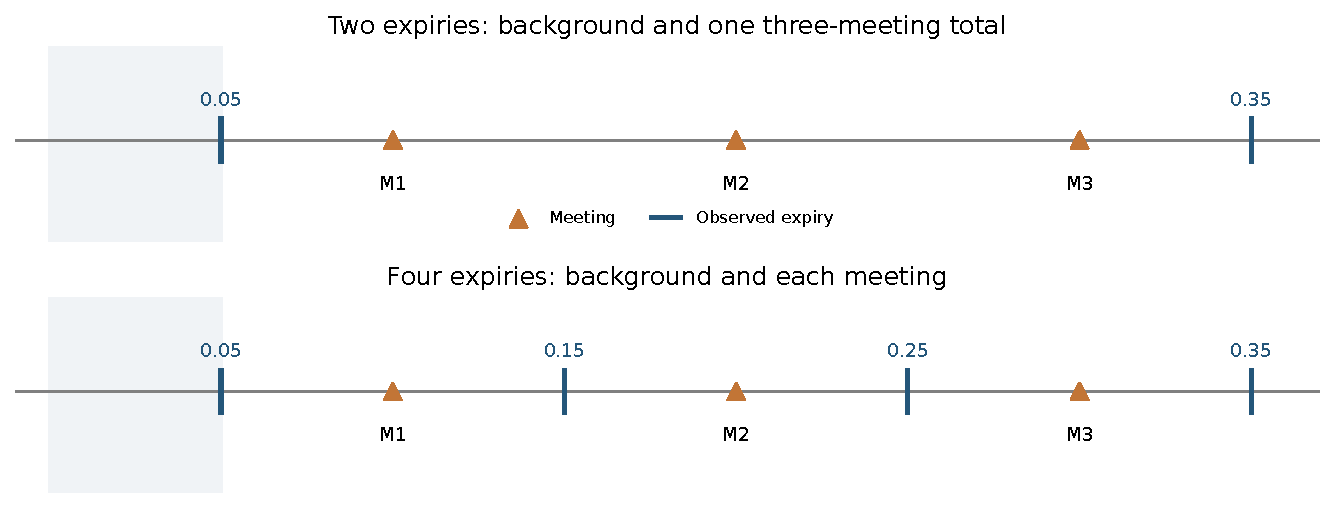
\includegraphics[width=.94\textwidth]{figures/calendar.pdf}
\caption{An expiry between meetings adds an independent variance observation. With constant background variance, the first meeting-free interval identifies the background. The sparse calendar identifies only the sum of the three meeting variances; the denser calendar separates them. Time is measured in years.}\label{fig:calendar}
\end{figure}

\subsection{Known maturity-dependent background loadings}\label{sec:shape}
A parallel diffusion is convenient but is not necessary for the calendar argument. Suppose its loading at time $s$ on forward maturity $T$ is $\sigma(s)\phi(s,T)$, where $\phi$ is known, bounded, and jointly Borel measurable on the finite horizon. Replace the continuous part of \eqref{eq:curve} by
\begin{equation}\label{eq:shapecurve}
\int_0^t\sigma(s)\phi(s,T)\,\dd W_s
+\int_0^t\sigma(s)^2\phi(s,T)\left(\int_s^T\phi(s,x)\,\dd x\right)\dd s.
\end{equation}
The deterministic drift is again the HJM drift. The meeting part remains the parallel-jump specification already defined.

For contract $\ell$, define its average diffusion loading
\[
\beta_\ell(s)=\frac1{\delta_\ell}\int_{a_\ell}^{b_\ell}\phi(s,x)\,\dd x,
\qquad 0\leq s\leq S_\ell.
\]
Its normalized log variance becomes
\begin{equation}\label{eq:shapeD}
\cV_\ell=\sum_{T_i\leq S_\ell}v_i+\sum_j\mathsf D_{\ell j}u_j,\qquad
\mathsf D_{\ell j}=\int_{[c_{j-1},c_j)\cap(0,S_\ell]}\beta_\ell(s)^2\,\dd s.
\end{equation}
Set $\mathsf D_{0j}=0$ and $\Delta \mathsf D_{\ell j}=\mathsf D_{\ell j}-\mathsf D_{\ell-1,j}$.

\begin{corollary}[Calendar criterion with a known shape]\label{cor:shape}
For \eqref{eq:shapeD}, Theorem~\ref{thm:rank} holds with $\Lambda_E$ replaced by $(\Delta \mathsf D_{\ell j})_{\ell\in E,j}$. In particular, for the strictly increasing expiry sequence considered here, at least $n_b$ meeting-free gaps remain necessary.
\end{corollary}
When adjacent options refer to different accrual windows, the differenced background row is not just the variance accumulated between their expiries. Earlier Brownian shocks can have different weights in the two contracts. Some coefficients in $\Delta\mathsf D$ can therefore be negative. For example, with $\phi(s,T)=e^{-\kappa(T-s)}$, $\kappa>0$,
\[
\beta_\ell(s)=\frac{1-e^{-\kappa\delta_\ell}}{\kappa\delta_\ell}
                  e^{-\kappa(a_\ell-s)}.
\]
Moving the underlying window farther out reduces the weight of an earlier shock. One must build $\mathsf D$ from the actual underlying windows before differencing. The corollary treats a known $\phi$; estimating its shape parameters creates an additional inverse problem. With several windows at the same expiry, build a row for each contract directly in \eqref{eq:shapeD}. Such rows have identical meeting entries but can have different background entries. They can therefore add background information under a nonparallel known shape, even though they add no new meeting cutoff.

\subsection{What futures quotes add}\label{sec:extra}
Theorem~\ref{thm:rank} deliberately uses only $\cV$. Proposition~\ref{prop:pricing} shows why a statement about all option and futures prices would be different. For the parallel diffusion and pre-accrual expiry,
\begin{equation}\label{eq:zrows}
\frac{z_\ell}{\delta_\ell}
=\sum_i(S_\ell-T_i)^+v_i+
  \sum_ju_j\int_{[c_{j-1},c_j)\cap(0,S_\ell]}(S_\ell-s)\,\dd s.
\end{equation}
The mean fitted from the cash option surface, together with its underlying futures quote, supplies this additional row. Known initial bond prices can supply the $p$ rows of \eqref{eq:p}. Full rank of the stacked observation matrix is the appropriate exact identification test for those richer data.

\begin{table}[ht]
\centering\small
\begin{tabular}{p{.34\textwidth}p{.56\textwidth}}
\toprule
Observations used & Model quantities available in the exact experiment\\
\midrule
Option-variance panel & $q_\ell$, hence $\cV_\ell$; calendar criterion applies directly.\\
Complete cash option surfaces & $P(0,S_\ell)$, $m_\ell$, and $q_\ell$.\\
Surfaces plus underlying futures & Additionally $z_\ell=\log G_{0,\ell}-\log m_\ell$.\\
Surfaces, futures, initial bond curve & Additionally $p_\ell=\log G_{0,\ell}-\int_{a_\ell}^{b_\ell}f_0$.\\
\bottomrule
\end{tabular}
\caption{Different observation sets require different identification claims. With a known initial curve, the two strikes in Proposition~\ref{prop:finitequotes} can replace each complete surface in this exact experiment. Finite price precision still requires bounds.}\label{tab:observations}
\end{table}

The extra information may be tiny in rate-price units. Move $100$ bp$^2$ of variance between two meetings separated by $1/12$ year while preserving the total. At a later expiry, \eqref{eq:zrows} changes $z$ by $\delta\times10^{-6}/12$. For a quarterly window this is about $2.1\times10^{-8}$. Holding $G_0$ fixed, the corresponding shift in the mean rate is about $G_0\times0.00083$ bp. With a known initial curve, the futures mean can also move, but on the same small scale for this perturbation. Exact nonzero information is not necessarily informative at a quarter-basis-point price tolerance. This arithmetic illustrates conditioning, not a general bound for every parameter direction.

Futures alone can identify in a deliberately designed pure-jump experiment. Suppose background volatility is zero and use windows $a_n=T_n<b_n<T_{n+1}$ (with $b_N>T_N$). Subtract the known initial-curve integral from $\log G_{0,n}$ to obtain $p_n$. Then
\[
v_n=\frac{p_n-\delta_n\sum_{i<n}(b_n-T_i)v_i}{\delta_n^2},\qquad
\delta_n=b_n-T_n.
\]
The coefficients are triangular because a later meeting occurs after the window ends. This identifies all meeting variances recursively. Standard quarterly futures do not supply these freely chosen windows. The result distinguishes insufficient instruments from an intrinsic inability of futures prices to contain variance information.

Appendix~\ref{app:listedcalendar} applies the rank criterion to actual versus hypothetical listing calendars. It also exhibits a known exponential loading for which an otherwise identifying background partition becomes singular at one positive decay rate, and a case where futures-mean observations restore exact rank while adding information far below the price tolerance. These examples are useful checks before interpreting a numerically unique calibration.
